

%%%%%%%%%%%%%%%%%%%%%%%%%%%%%%%%%%%%%%%%%
% Journal Article
% LaTeX Template
% Version 1.4 (15/5/16)
%
% This template has been downloaded from:
% http://www.LaTeXTemplates.com
%
% Original author:
% Frits Wenneker (http://www.howtotex.com) with extensive modifications by
% Vel (vel@LaTeXTemplates.com)
%
% License:
% CC BY-NC-SA 3.0 (http://creativecommons.org/licenses/by-nc-sa/3.0/)
%
%%%%%%%%%%%%%%%%%%%%%%%%%%%%%%%%%%%%%%%%%

%----------------------------------------------------------------------------------------
%	PACKAGES AND OTHER DOCUMENT CONFIGURATIONS
%----------------------------------------------------------------------------------------

\documentclass[10pt]{article} % Single column

%\documentclass[twoside,twocolumn]{article} % Two column

\usepackage{blindtext} % Package to generate dummy text throughout this template 

\usepackage[sc]{mathpazo} % Use the Palatino font
\usepackage[T1]{fontenc} % Use 8-bit encoding that has 256 glyphs
\linespread{1.05} % Line spacing - Palatino needs more space between lines
\usepackage{microtype} % Slightly tweak font spacing for aesthetics

\usepackage[english]{babel} % Language hyphenation and typographical rules

\usepackage{algorithm}
	
\usepackage[hmarginratio=1:1,top=32mm,columnsep=20pt]{geometry} % Document margins
\usepackage[hang, small,labelfont=bf,up,textfont=it,up]{caption} % Custom captions under/above floats in tables or figures
\usepackage{booktabs} % Horizontal rules in tables

\usepackage{lettrine} % The lettrine is the first enlarged letter at the beginning of the text

\usepackage{enumitem} % Customized lists
\setlist[itemize]{noitemsep} % Make itemize lists more compact

\usepackage{abstract} % Allows abstract customization
\renewcommand{\abstractnamefont}{\normalfont\bfseries} % Set the "Abstract" text to bold
\renewcommand{\abstracttextfont}{\normalfont\small\itshape} % Set the abstract itself to small italic text

\usepackage{titlesec} % Allows customization of titles
\renewcommand\thesection{\Roman{section}} % Roman numerals for the sections
\renewcommand\thesubsection{\roman{subsection}} % roman numerals for subsections
\titleformat{\section}[block]{\large\scshape\centering}{\thesection.}{1em}{} % Change the look of the section titles
\titleformat{\subsection}[block]{\large}{\thesubsection.}{1em}{} % Change the look of the section titles

\usepackage{fancyhdr} % Headers and footers
\pagestyle{fancy} % All pages have headers and footers
\fancyhead{} % Blank out the default header
\fancyfoot{} % Blank out the default footer
\fancyhead[C]{Alternative Topic Modeling Optative Course. \textbf{Study of LDA Method}} % Custom header text
\fancyfoot[RO,LE]{\thepage} % Custom footer text

\usepackage{titling} % Customizing the title section

\usepackage{hyperref} % For hyperlinks in the PDF

\usepackage{graphicx} % For images

\usepackage{pifont} % bullets

\usepackage{amsmath}

\usepackage{algpseudocode}

\usepackage{lipsum}

% Keywords command
\providecommand{\keywords}[1]
{
	\small	
	\vspace{0.5em}
	\noindent \textbf{\textit{Keywords --- }} #1
}


%----------------------------------------------------------------------------------------
%	TITLE SECTION
%----------------------------------------------------------------------------------------

\setlength{\droptitle}{-4\baselineskip} % Move the title up

\pretitle{\begin{center}\Huge\bfseries} % Article title formatting
	\posttitle{\end{center}} % Article title closing formatting
\title{\normalsize{Alternative Topic Modeling Optative Course}\\
	\Huge\bfseries Study of LDA Method \\
} % Article title
\author{% 
	Laura Victoria Riera P\'erez\\
	Mari\'e del Valle Reyes \vspace{1em} \\
	\small Senior year. Computer Science. \\ % institution
	\small School of Math and Computer Science, University of Havana, Cuba \\ % institution
}
\date{\footnotesize \today } % Leave empty to omit a date


% Abstract configurations
\renewenvironment{abstract}
{\small
	\begin{center}
		\bfseries \abstractname\vspace{-.5em}\vspace{0pt}
	\end{center}
	\list{}{
		\setlength{\leftmargin}{1.5cm}%
		\setlength{\rightmargin}{\leftmargin}%
	}%
	\item\relax}
{\endlist}

\usepackage{amsthm}
\usepackage{amssymb}
\usepackage{todonotes} % \TODO
\usepackage{listings} % Code listings
\usepackage{xcolor}

\definecolor{backcolour}{rgb}{0.95,0.95,0.92}

\newcommand{\csl}[1]{\colorbox{backcolour}{\texttt{#1}}}

\newcommand{\imgcaption}[2]{\tiny \textbf{Figura #1.} #2.}

\newcommand{\mgc}[2][]{\colorbox{backcolour}{\texttt{\_\_#2\_\_#1}}}

\newcommand{\mgccapt}[1]{\texttt{\_\_#1\_\_}}

\newtheorem{thm}{Teorema}
\newtheorem{mydef}{Definici\'on}%[section]
\newtheorem{lem}{Lema}
\newtheorem{fig}{\scriptsize{Figura}}
\newtheorem{col}{Corolario}


\renewcommand{\qedsymbol}{\rule{0.7em}{0.7em}}

% Hyperlinks configurations
\hypersetup{
	colorlinks=true,
	linkcolor=black,
	filecolor=magenta,      
	urlcolor=cyan,
	pdftitle={Overleaf Example},
	pdfpagemode=FullScreen,
}

%----------------------------------------------------------------------------------------

\begin{document}
	% Print the title
	\maketitle
	
	%----------------------------------------------------------------------------------------
	%	ARTICLE CONTENTS
	%----------------------------------------------------------------------------------------
	\begin{abstract}
		\lipsum[1]
		
		\keywords{}
	\end{abstract}

	\section*{Project's repository}
	
	\begin{center}
		\href{https://github.com/computer-science-crows/study-of-lda-method}{https://github.com/computer-science-crows/study-of-lda-method}
	\end{center}
	
	\section{Initial Analysis}
	
	\subsection{Different coherence and perplexity}
	\todo{Poner que en las observaciones se observan diferentes valores de coherencia y perplexity e interpretar los resultados de acuerdo a eso.}
	In the LDA (Latent Dirichlet Allocation) model, coherence and perplexity can vary when running the model multiple times with the same set of words. This is due to the stochastic nature of the algorithm and the various factors that can influence the results.\todo[backgroundcolor=green, linecolor=black]{aqui se ve por qu\'e hay diferentes valores}
	
		
	\begin{center}
		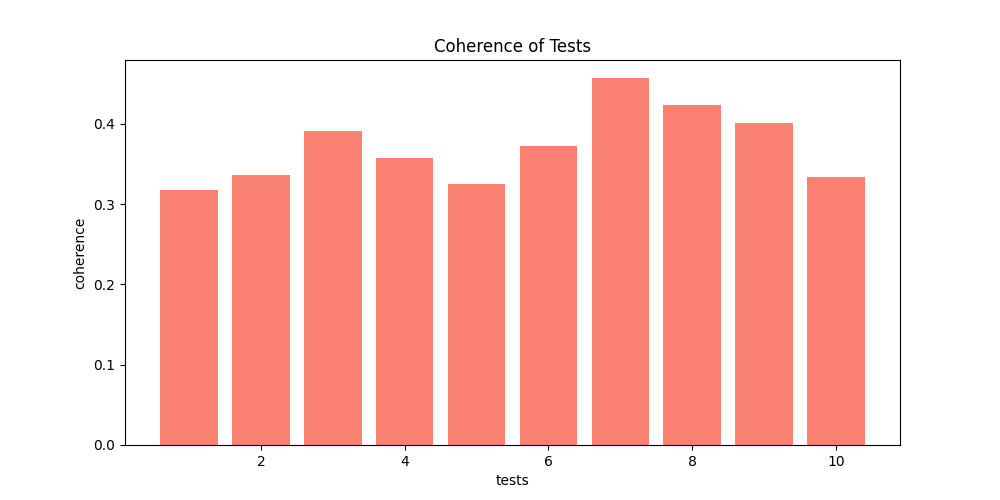
\includegraphics[width=7.5cm]{images/coherence_stopwords}
		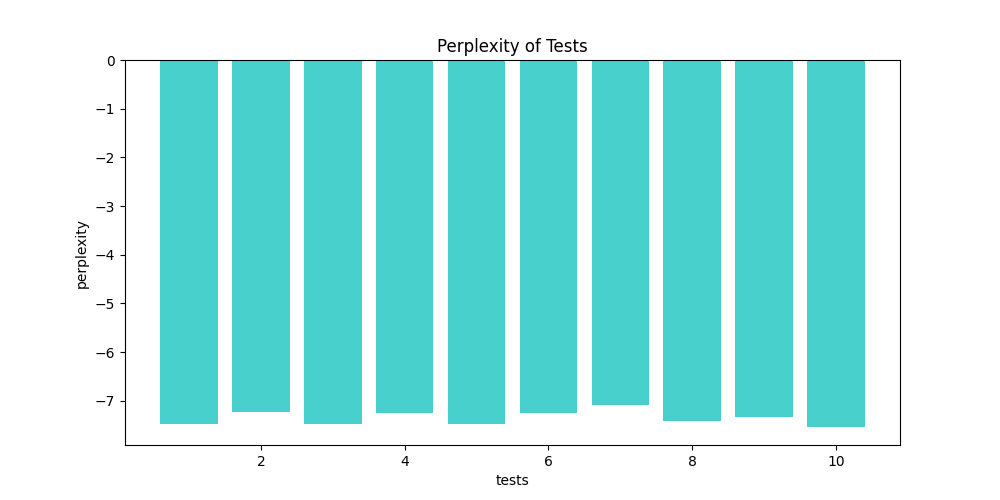
\includegraphics[width=7.5cm]{images/perplexity_stopwords}
	\end{center}

	\textit{Perplexity} is a measure used in LDA models to evaluate how well the model fits the data. A lower perplexity value indicates a better fit of the model. However, perplexity can vary across different model runs due to random initialization and the way topics are generated and words are assigned. Therefore, you may obtain different perplexity values each time you run the model with the same set of words.
	
	\textit{Coherence}, on the other hand, is a measure that assesses the coherence of the topics generated by the model. Coherence is based on the relationship between words within each topic and is used to determine how interpretable the topics are. Similar to perplexity, coherence can also vary across different model runs due to randomness and other factors.
	
	The variability in coherence and perplexity can be attributed to various factors, such as random initialization of the model, parameter selection, quality of the training corpus, and the amount of available data. Additionally, different implementations of LDA may have variations in how coherence and perplexity are calculated, which can also contribute to differences in results.
	
	It is important to note that both coherence and perplexity are approximate measures and do not provide a definitive evaluation of the quality of the LDA model. They should be used in conjunction with other evaluation techniques and analysis to gain a more comprehensive understanding of the model results.
	
	In summary, coherence and perplexity can vary when running the LDA model multiple times with the same set of words due to randomness and other factors involved in the algorithm. It is important to consider these variations and use other evaluation techniques to obtain a more complete picture of the model's quality.
	

	
	\subsection{Solution}
	\todo[backgroundcolor=green, linecolor=black]{Se dice una solucion para mejorar la variabilidad de valores}
	To address the issue of variability in coherence and perplexity in the LDA model when running it multiple times with the same set of words, the following strategies can be considered:
	\begin{enumerate}
		\item Adjust the model parameters: The parameters of the LDA model, such as the number of topics and training iterations, can influence the results. Adjusting these parameters might improve coherence and perplexity. You can experiment with different values and evaluate how they affect the results.
		
		\item Use a fixed random seed: Random initialization of the model can introduce variability in the results. By setting a fixed random seed before each model run, you can ensure consistent initializations and obtain more stable results.
		
		\item Increase the amount of training data: The amount of training data can also impact result stability. If you have a small set of words, variability may be higher. Consider adding more data or expanding the training corpus to achieve more consistent results.
		
		\item Perform averaging across multiple runs: Instead of relying on the results of a single model run, you can perform multiple runs and average the results. This can help reduce variability and obtain a more reliable estimate of coherence and perplexity.
		
		\item Use cross-validation techniques: Cross-validation is a technique that can evaluate the model's performance on different data partitions. By performing cross-validation, you can obtain a more robust measure of coherence and perplexity, as the model is evaluated on different subsets of data.
	\end{enumerate}

	It's important to note that while these strategies can help reduce variability in coherence and perplexity, there may still be some variation in the results. This is due to the stochastic nature of the algorithm and the inherent complexity of text data. It is recommended to evaluate the results from multiple runs and use other evaluation techniques to gain a more comprehensive understanding of the LDA model.
	
	\subsection{Test 8}
	\todo{Poner se tomo el test 8 como ejemplo, y se puede observar que la mayor\'ia de las palabras son stopwords, y analizar los valores de coherencia y perplexity.}
	La mayor\'ia de las palabras son stopwords.
	
	\begin{center}
		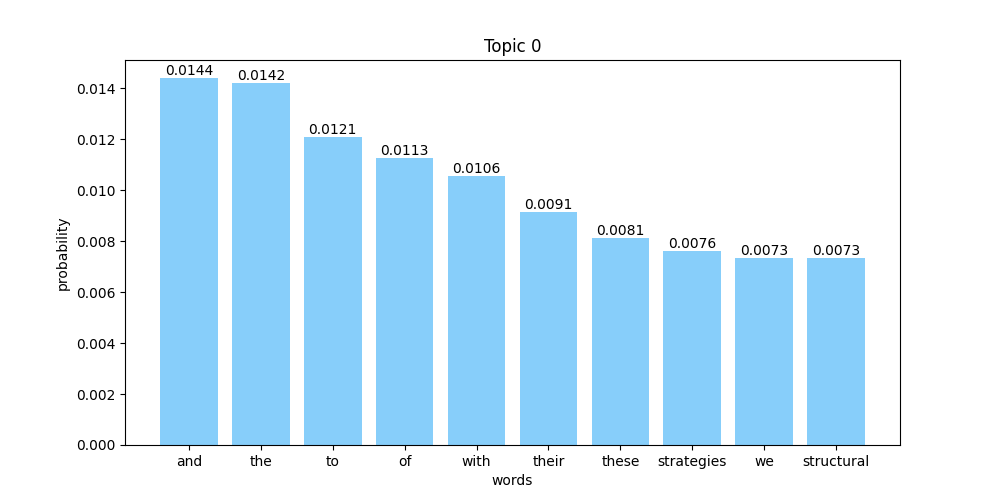
\includegraphics[width=7.5cm]{images/plots/test_8/topic_0.png}
		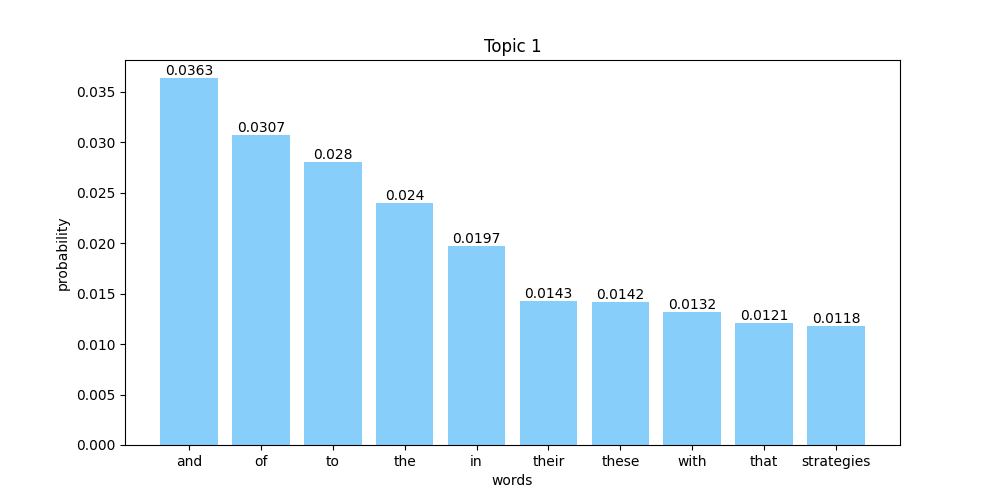
\includegraphics[width=7.5cm]{images/plots/test_8/topic_1.png}
		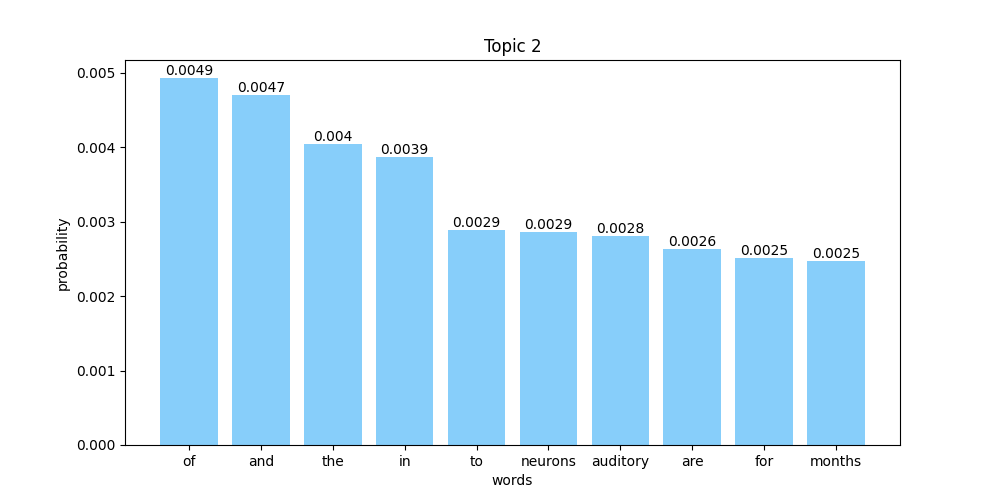
\includegraphics[width=7.5cm]{images/plots/test_8/topic_2.png}
		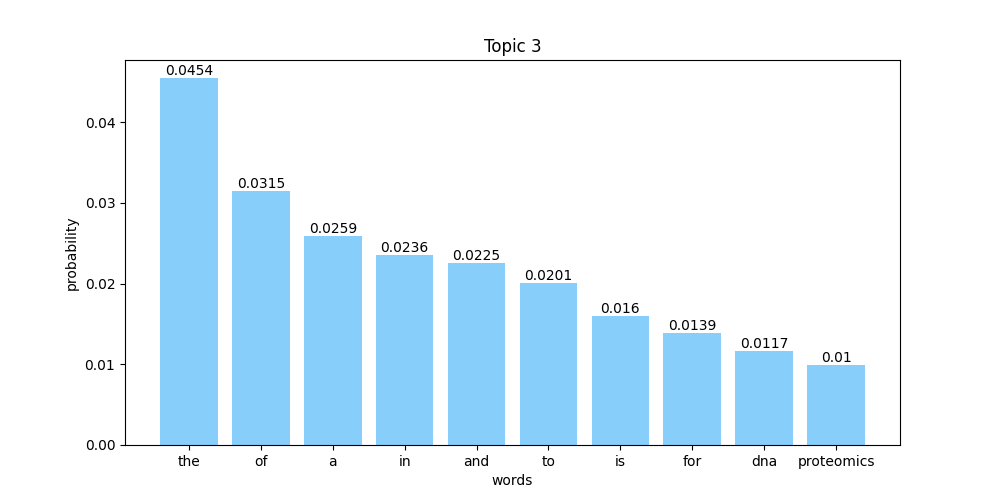
\includegraphics[width=7.5cm]{images/plots/test_8/topic_3.png}
		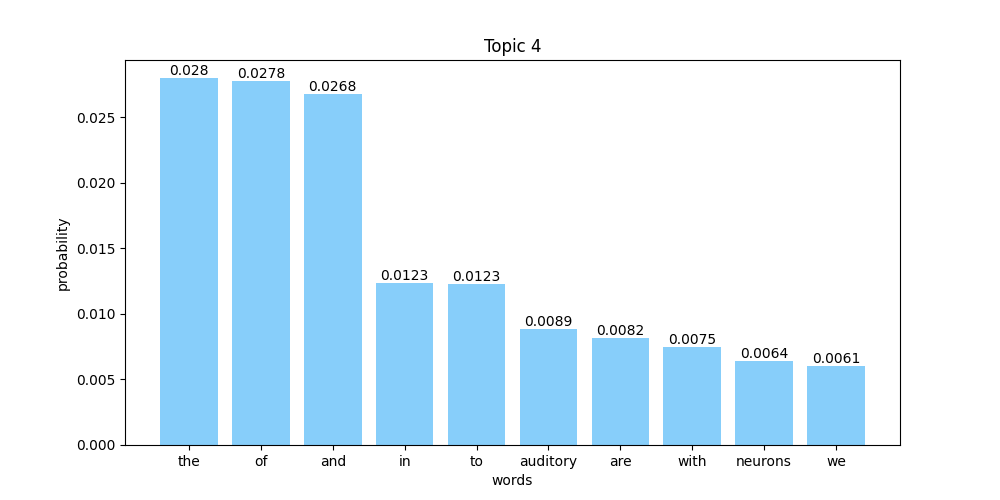
\includegraphics[width=7.5cm]{images/plots/test_8/topic_4.png}
		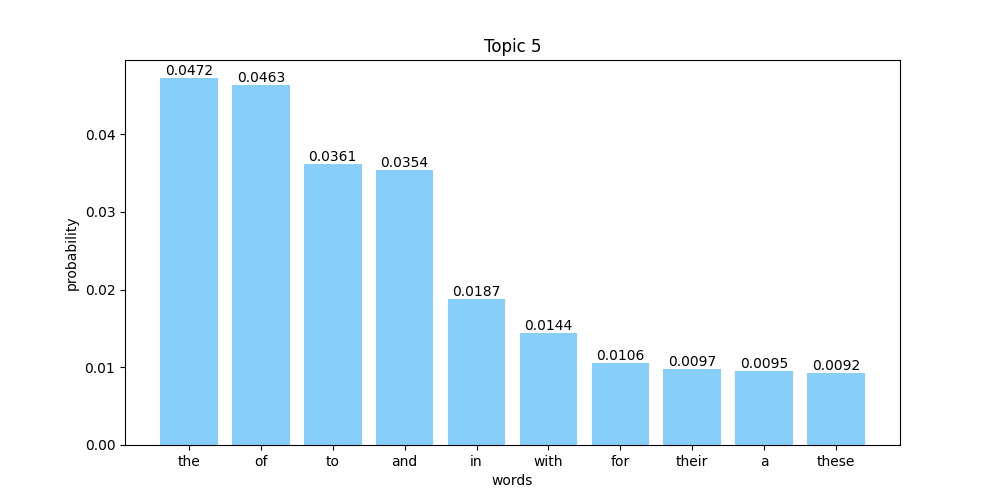
\includegraphics[width=7.5cm]{images/plots/test_8/topic_5.png}
		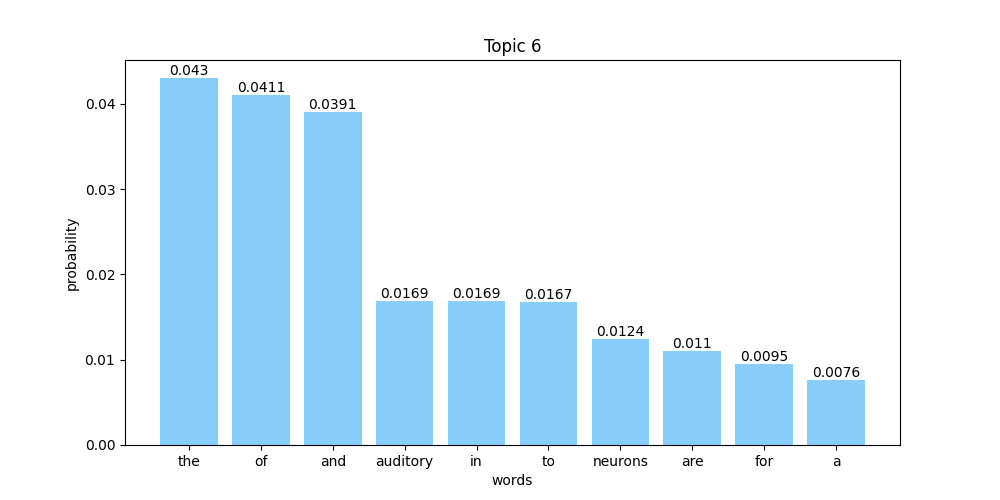
\includegraphics[width=7.5cm]{images/plots/test_8/topic_6.png}
		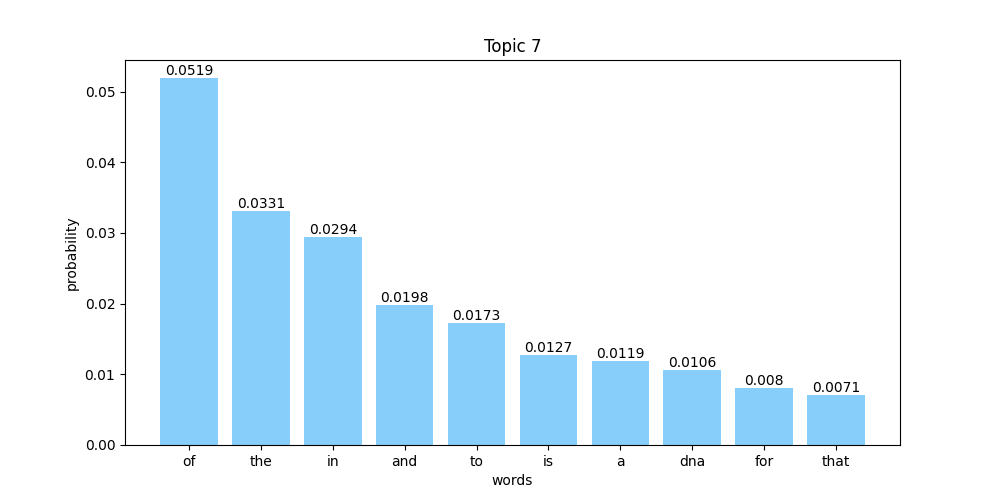
\includegraphics[width=7.5cm]{images/plots/test_8/topic_7.png}
	\end{center}

	La perplexity es -7.255103257328984, y la coherencia  0.3718197713201331.
	
	\section{Stopwords}
	\todo[backgroundcolor=green, linecolor=black]{Explicaci\'on de stopwords}
	Stop words are commonly used words in a language that are often considered insignificant or carry little meaning in the context of natural language processing (NLP) and text mining. These words are typically articles, prepositions, conjunctions, or pronouns. Examples of stop words in English include "a", "the", "is", "are", and so on. Stop words are used to eliminate words that are so commonly used that they may not contribute much to the analysis or understanding of text data.
	
	\todo{2.a Poner que la mayor\'ia de las palabras son stopwords y buscar por qu\'e esto sucede}
	\subsection{Removing stopwords}
	
	The removal of stopwords is a common step in data preparation for topic modeling with LDA (Latent Dirichlet Allocation). Stopwords are highly common and frequent words in a given language, such as "the," "and," "of," "to," etc. These words do not contribute much meaning or relevant information for topic identification and can negatively affect the quality of LDA results.
	
	Here are some reasons why stopwords should be removed when performing LDA:
	\begin{enumerate}
		\item Noise reduction: By eliminating stopwords, the noise in the data is reduced. Stopwords are words that are so common that they appear in almost every document and do not provide distinctive information about topics. Removing them reduces the amount of irrelevant words in the analysis and focuses on the most significant words for topic identification.
		
		\item 	Improved topic interpretability: Removing stopwords enhances the interpretability of topics generated by the LDA model. Stopwords tend to appear in multiple topics and do not help clearly distinguish the themes. By removing them, the most relevant and distinctive keywords of each topic are highlighted, making interpretation and analysis easier.
		
		\item Dimensionality reduction: Removing stopwords reduces the dimensionality of the word space used for topic modeling. This can help improve computational efficiency and reduce memory consumption. By eliminating highly frequent yet uninformative words, a more compact and efficient representation of documents can be achieved.
	\end{enumerate}
	
	Stopword removal can be performed using pre-defined lists of stopwords specific to each language. These lists contain common words that are considered stopwords and can be easily found online. For example, for the Spanish language, you can find stopwords lists containing words like "el," "y," "de," etc.

	In summary, removing stopwords in the LDA process is important to reduce noise in the data, improve topic interpretation, and reduce the dimensionality of the word space. This helps obtain more accurate and meaningful results in topic modeling with LDA
	

	
	\subsection{Code Modification}
	
	Se creo un nuevo .py en donde se descomentaron las lineas de c\'odigo que se encargaban de eliminar las stopwords del conjunto de palabras dado en TokenVieuxM.txt.
	
	\begin{center}
		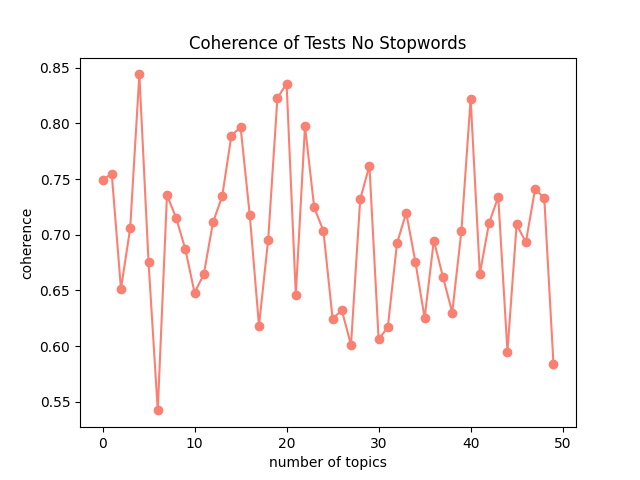
\includegraphics[width=7.5cm]{images/coherence_no_stopwords}
		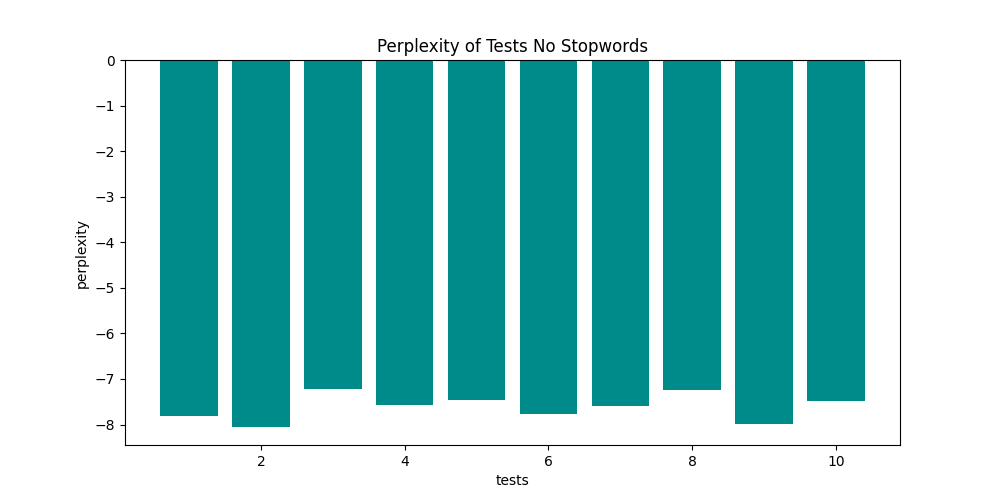
\includegraphics[width=7.5cm]{images/perplexity_no_stopwords}
	\end{center}

	\subsubsection{Test 8 No Stopwords}\label{test_8_ns_1}
	
	\begin{center}
		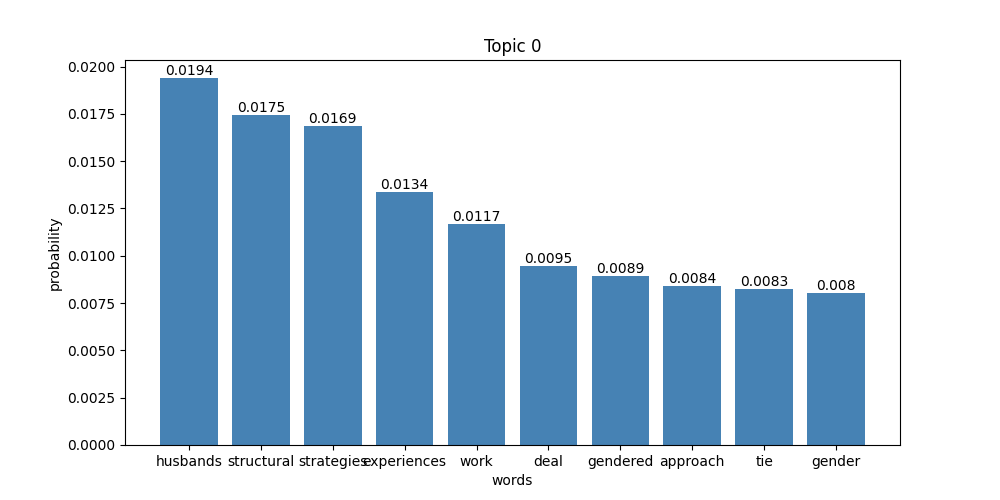
\includegraphics[width=7.5cm]{images/plots/test_8_no_stopwords/topic_0.png}
		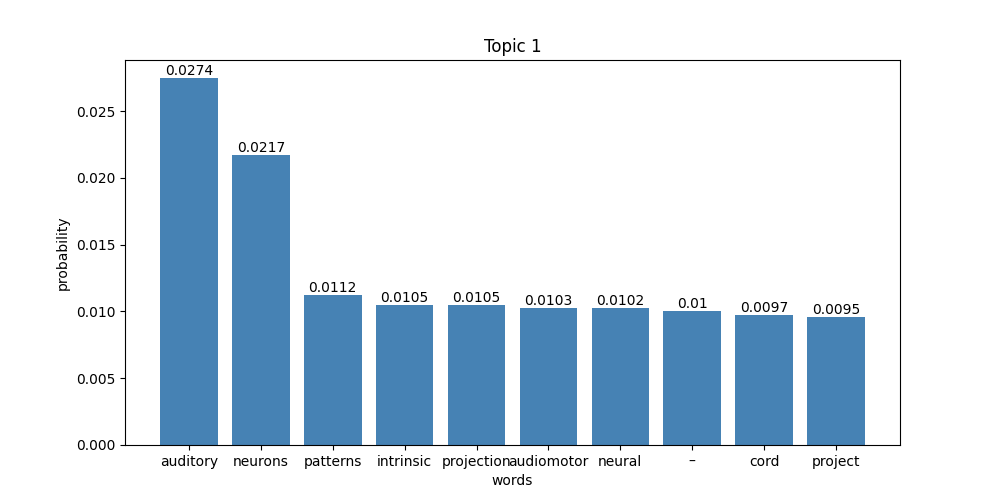
\includegraphics[width=7.5cm]{images/plots/test_8_no_stopwords/topic_1.png}
		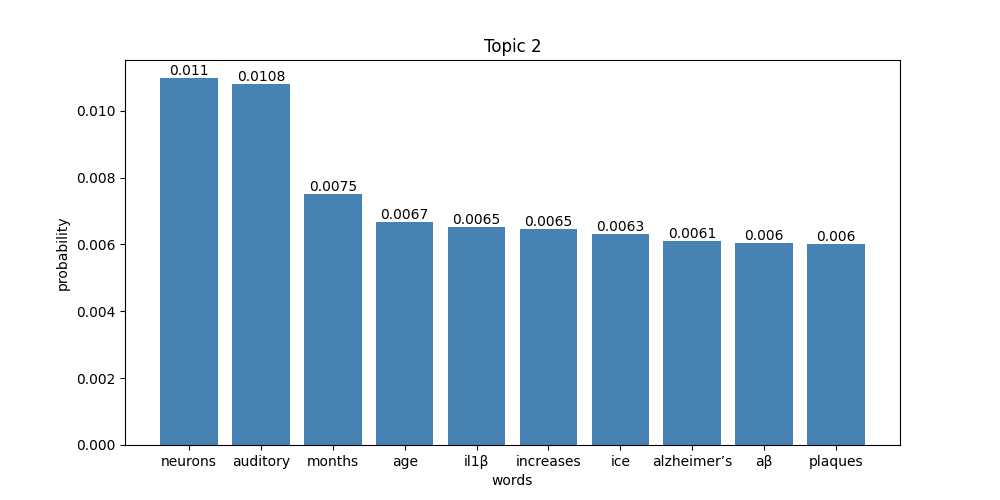
\includegraphics[width=7.5cm]{images/plots/test_8_no_stopwords/topic_2.png}
		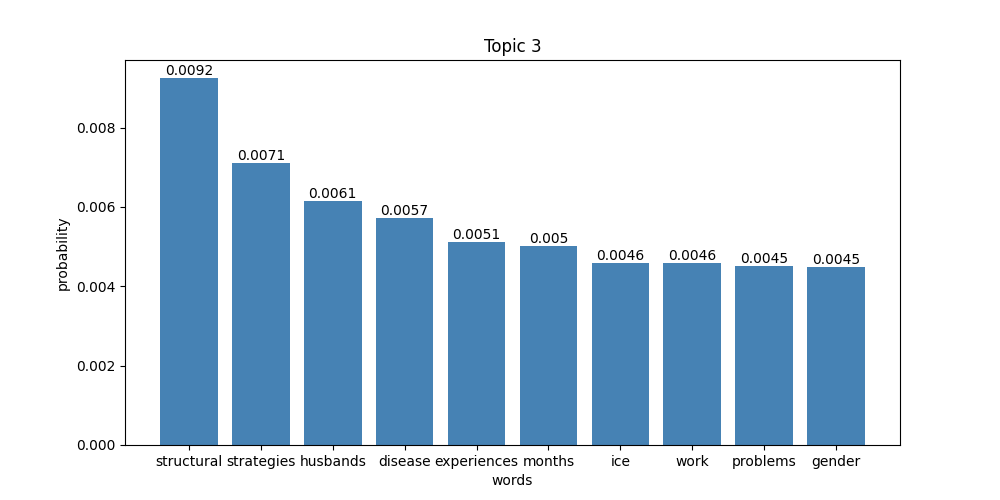
\includegraphics[width=7.5cm]{images/plots/test_8_no_stopwords/topic_3.png}\
		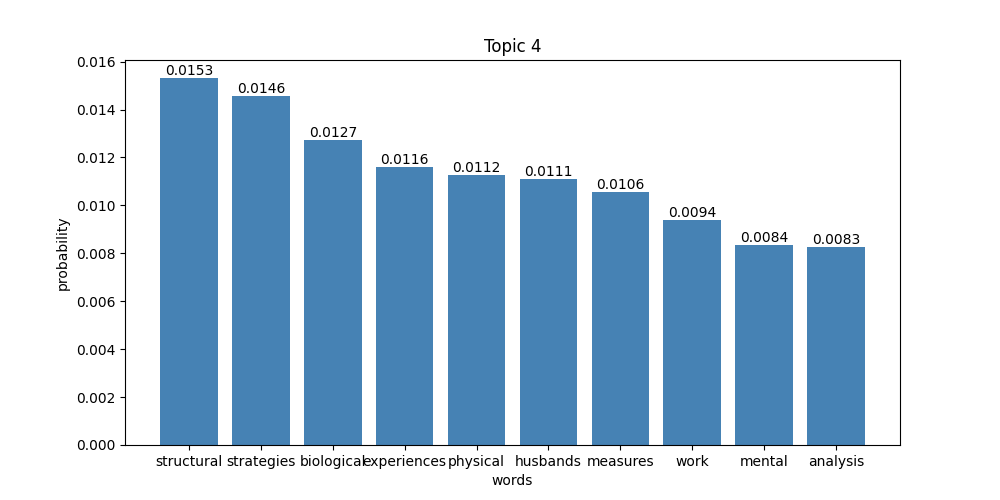
\includegraphics[width=7.5cm]{images/plots/test_8_no_stopwords/topic_4.png}
		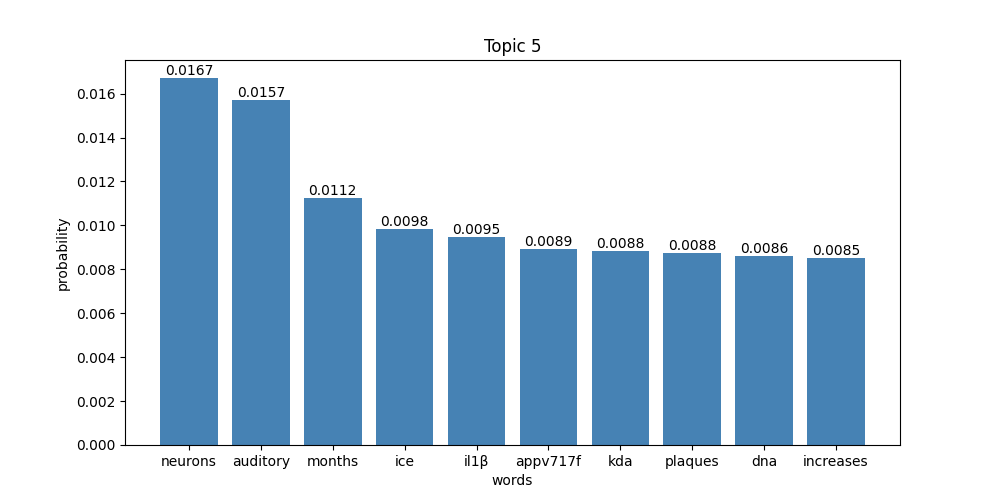
\includegraphics[width=7.5cm]{images/plots/test_8_no_stopwords/topic_5.png}
		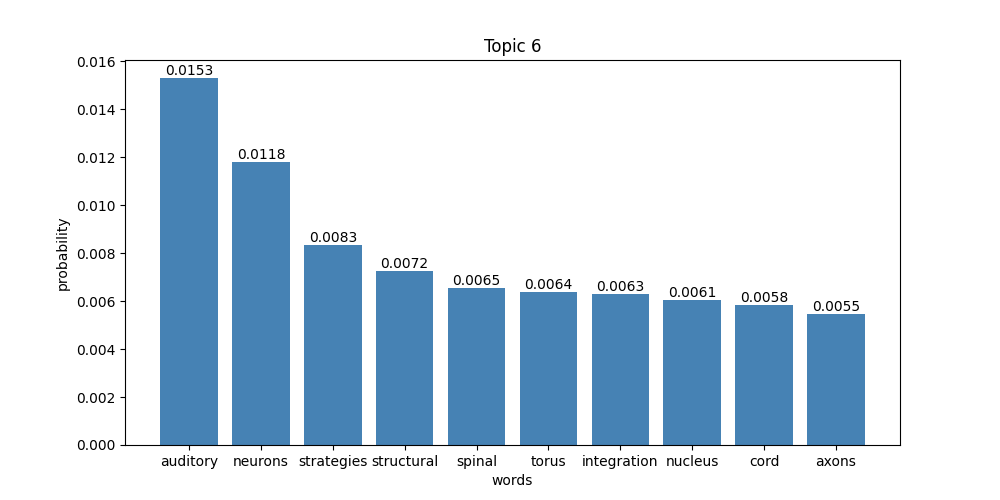
\includegraphics[width=7.5cm]{images/plots/test_8_no_stopwords/topic_6.png}
		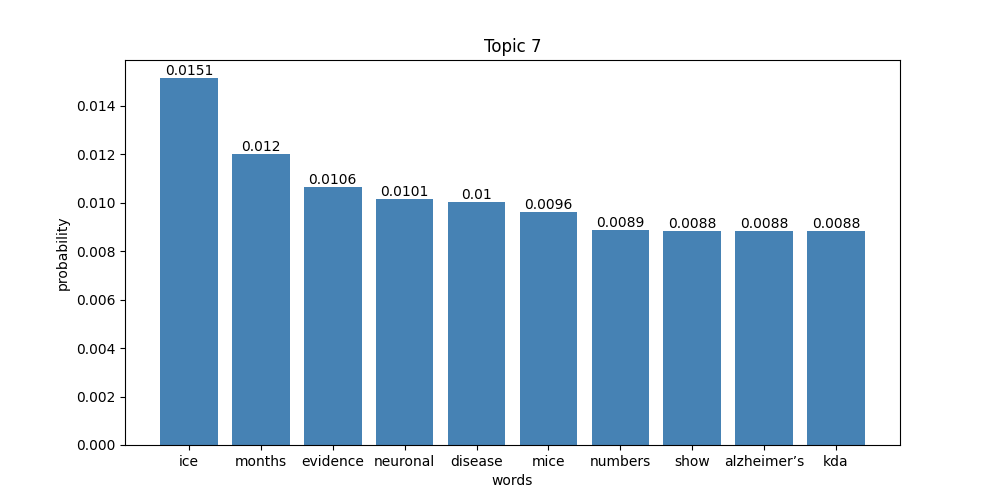
\includegraphics[width=7.5cm]{images/plots/test_8_no_stopwords/topic_7.png}
		
		
	\end{center}

	La perplexity es -7.764361092424768 y la coherencia  0.6284575950301475.

	\todo{2.c hay que comparar los resultados con el test sin remover stopwords y ver la relaci\'on entre coherencia y perplexity}
	
	\subsection{Changing number of topics}
	\todo{2.d Escribir cual ser\'ia el n\'umero \'optimo de t\'opicos y por qu\'e}
	\begin{center}
		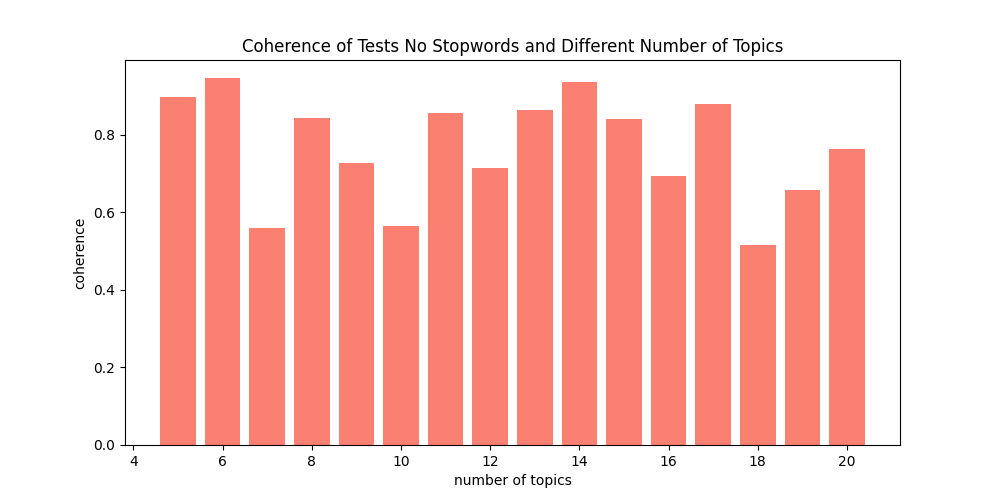
\includegraphics[scale=0.6]{images/coherence_no_stopwords_diff_n_topics}
		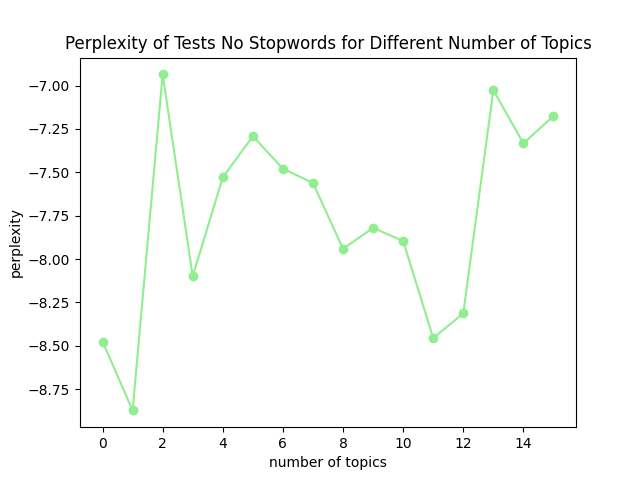
\includegraphics[scale=0.6]{images/perplexity_no_stopwords_diff_n_topics}
	\end{center}

	El n\'umero \'optimo de t\'opicos de acurdo a los valores de coherencias deber\'ia ser 6.
	
	
	
	\section{Dataset 2}
		\todo{2.e Comparar los resultados de este dataset con el \ref{test_8_ns_1} y llegar a conclusiones.}
	\begin{center}
		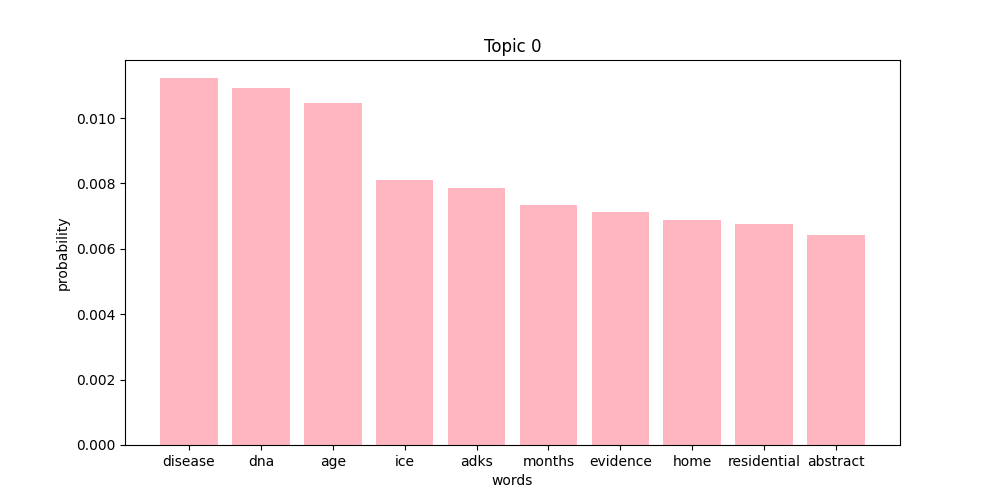
\includegraphics[width=7.5cm]{images/plots/test_8_no_stopwords_dataset_2/topic_0.png}
		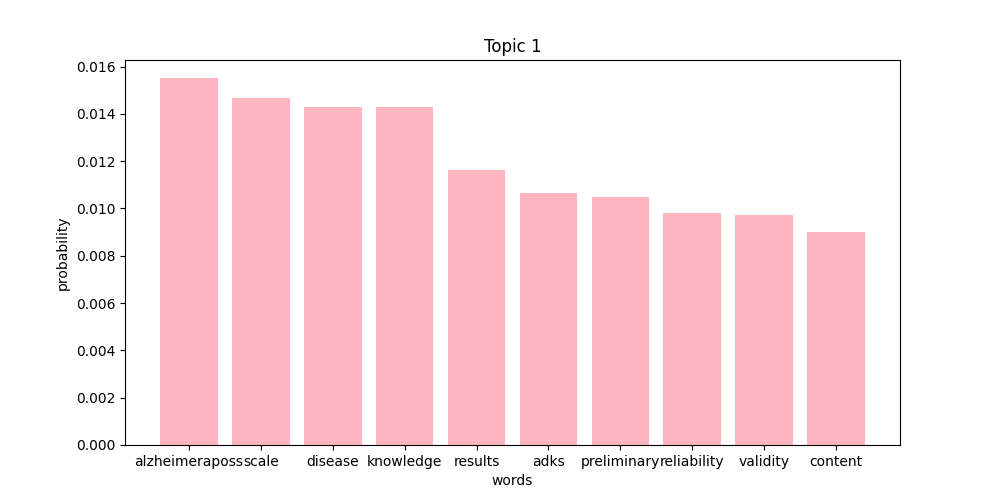
\includegraphics[width=7.5cm]{images/plots/test_8_no_stopwords_dataset_2/topic_1.png}
		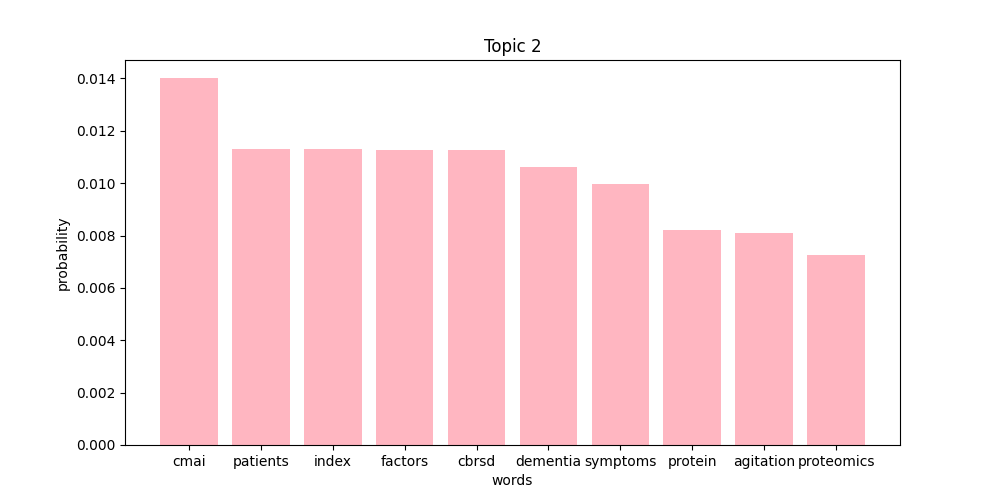
\includegraphics[width=7.5cm]{images/plots/test_8_no_stopwords_dataset_2/topic_2.png}
		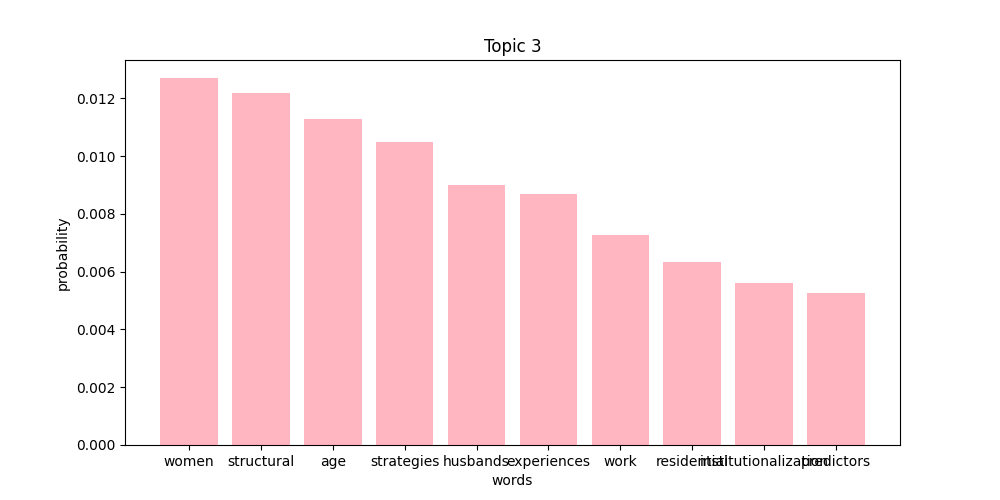
\includegraphics[width=7.5cm]{images/plots/test_8_no_stopwords_dataset_2/topic_3.png}\
		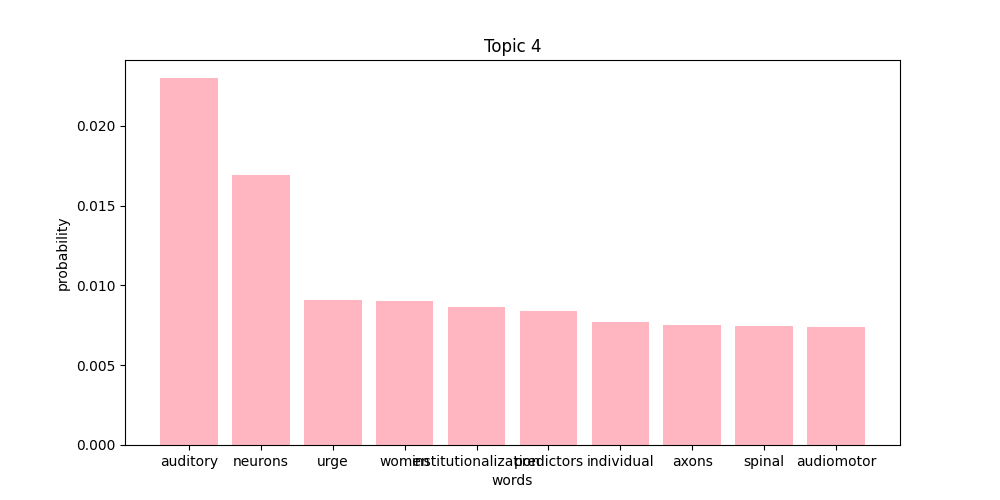
\includegraphics[width=7.5cm]{images/plots/test_8_no_stopwords_dataset_2/topic_4.png}
		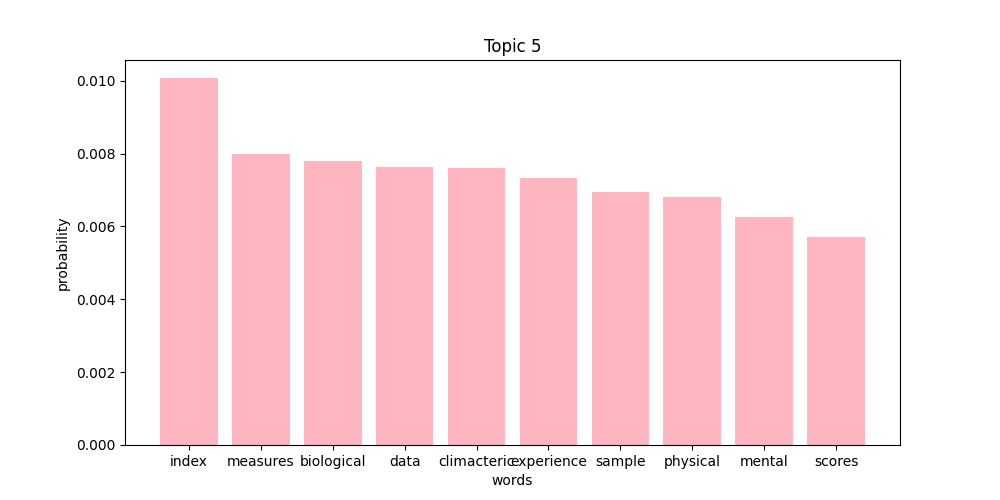
\includegraphics[width=7.5cm]{images/plots/test_8_no_stopwords_dataset_2/topic_5.png}
		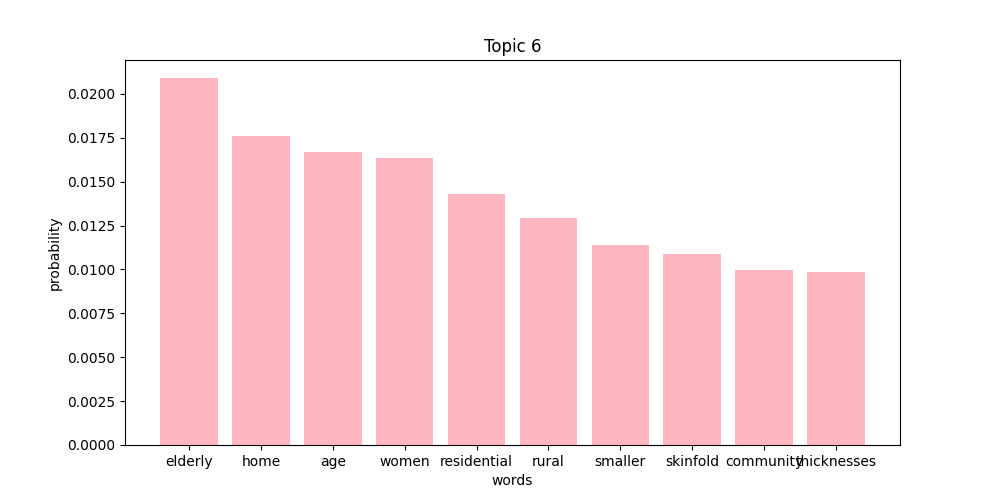
\includegraphics[width=7.5cm]{images/plots/test_8_no_stopwords_dataset_2/topic_6.png}
		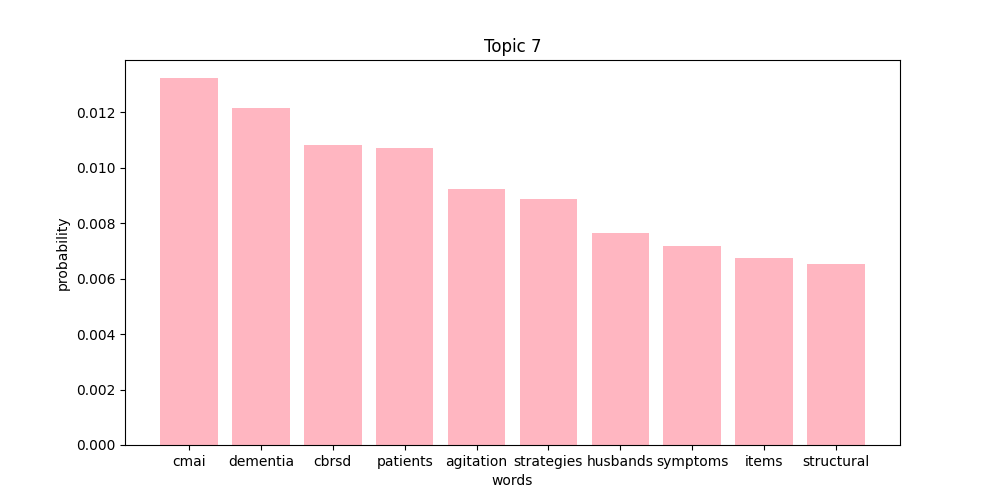
\includegraphics[width=7.5cm]{images/plots/test_8_no_stopwords_dataset_2/topic_7.png}	
		
	\end{center}

	\begin{center}
		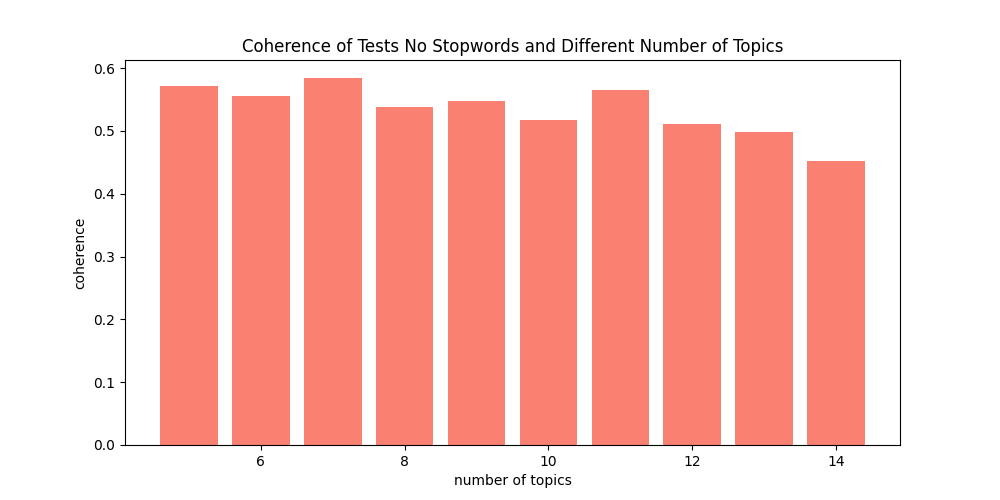
\includegraphics[width=7.5cm]{images/coherence_no_stopwords_2}
		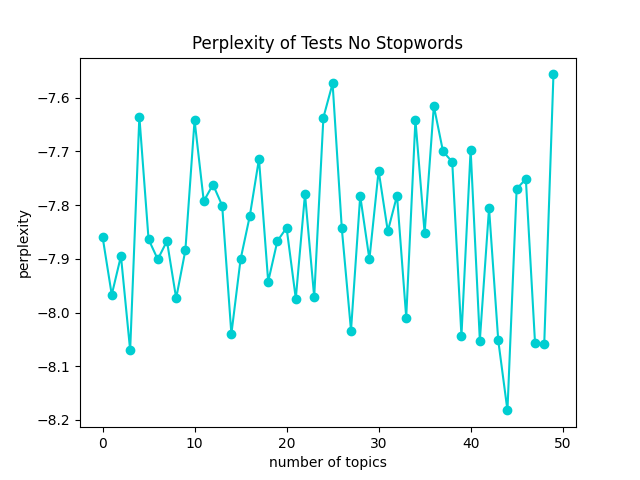
\includegraphics[width=7.5cm]{images/perplexity_no_stopwords_2}
	\end{center}


	\subsection{Different number of topics}
	\todo{2.f Analizar cu\'al es el n\'umero de t\'opicos \'optimo y justificar}
	\begin{center}
		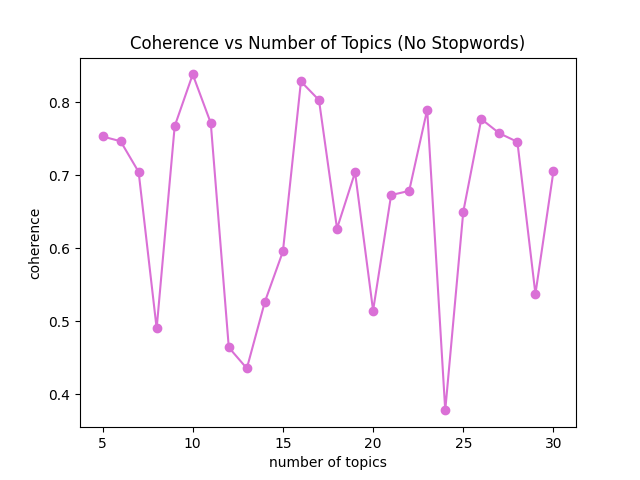
\includegraphics[width=7.5cm]{images/coherence_no_stopwords_diff_n_topics_2}
		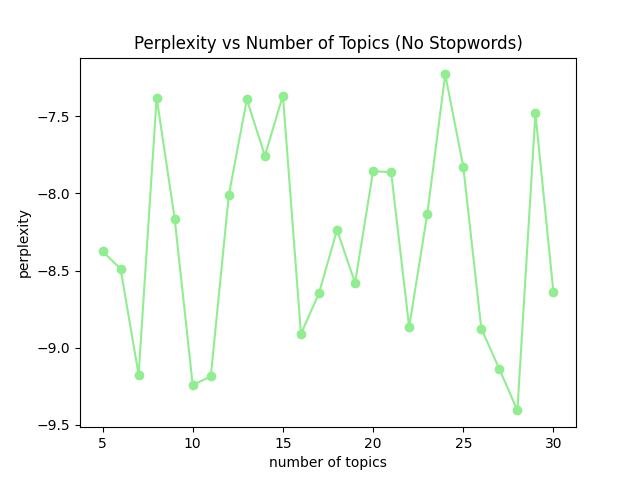
\includegraphics[width=7.5cm]{images/perplexity_no_stopwords_diff_n_topics_2}
	\end{center}
	
	\section{Most typical documents for topics}
	\todo{Ver como utilizar el m\'etodo}
	Para identificar el documento más típico en cada tópico utilizando LDA de Gensim en Python, puedes utilizar el método get\_document\_topics proporcionado por la clase LdaModel. Este método devuelve una lista de tuplas que contienen el ID del tópico y la probabilidad de ese tópico para cada documento.
	
	
	
	\begin{thebibliography}
		a
		\bibitem{introduction} Cormen, Thomas H. y otros. \emph{Introduction to Algorithms}. 
		The MIT Press.
		4ta Edici\'on.		
		Cambridge, Massachusetts.
		2022.
	\end{thebibliography}
\end{document}


